\section{Layer~3 – From Connections to Meaningful Groups}
\label{sec:layer3}

% ----- SUPERKRACHT -----
\begin{tcolorbox}[colback=blue!5, colframe=blue!60, title=\textbf{Superpower: The Grouper}]
\begin{center}
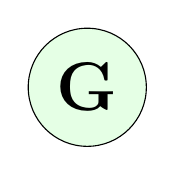
\begin{tikzpicture}
  \node[draw, circle, fill=green!10, minimum size=1.5cm, font=\bfseries\Huge] {G};
\end{tikzpicture}
\textit{“Which pieces belong together?”}
\end{center}
\end{tcolorbox}

Once the social network is drawn, you naturally notice groups: the
sports club, the music band, the chess team.  In the same way, Pixel
now looks for \emph{clusters} – groups of pixels that are so tightly
interlinked that they form a single, functional unit.

\begin{tcolorbox}[colback=yellow!5, colframe=yellow!80, title=Real‑life analogy]
A football team.  Eleven players move in patterns that are much more
coordinated among themselves than with the audience.  If you remove the
goalkeeper, the whole team’s performance drops dramatically.  Apeiron
uses this same logic to decide whether a cluster is important: it
temporarily deletes the cluster and checks if the system becomes
“blind” without it.
\end{tcolorbox}

\textbf{Pixel discovers shapes.}
Pixel finds a tight cluster of pixels in its web.  When it removes that
cluster, it can no longer tell the difference between a picture of the
rover and a picture of empty desert.  The cluster must be doing
something useful!  Without ever hearing the word “wheel” or “antenna”,
Pixel has discovered a \textbf{functional unit}: a reusable pattern
that helps it organise its visual world.

\begin{figure}[ht]
\centering
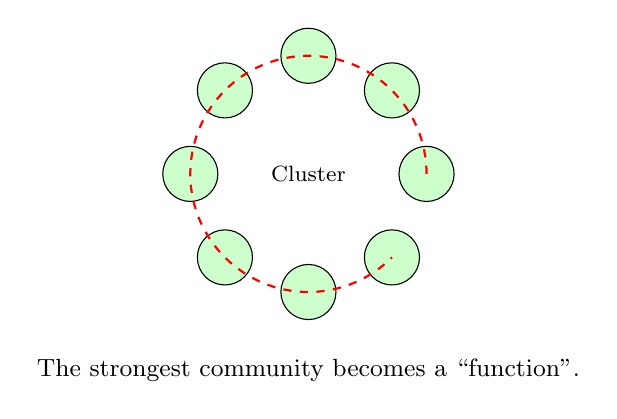
\begin{tikzpicture}[
    c/.style={circle, draw=black, fill=green!20, minimum size=0.7cm}
]
\foreach \i in {0,...,7} {
    \node[c] at (360/8*\i:1.5) {};
}
\node at (0,0) {\footnotesize Cluster};
\draw[red, thick, dashed] (360/8*0:1.5) arc (0:315:1.5);
\node at (0,-2.5) {\small The strongest community becomes a “function”.};
\end{tikzpicture}
\caption{Community detection: tight groups emerge from the network.}
\label{fig:clusters}
\end{figure}

This is a profound moment: Pixel begins to \emph{name} things – not
with human words, but with internal tags that mean “that pattern that
helps me predict what will happen next”.  Knowledge is born.

\subsection*{The ablation test – Pixel’s way of asking “are you important?”}

To check whether a cluster really matters, Pixel performs a
\emph{counterfactual ablation test}: it deletes the cluster from its
memory and tries to do the same tasks as before.  If the performance
drops sharply, the cluster was crucial; if nothing changes, it was
probably just noise.

Imagine you are trying to recognise a friend’s face.  If I erase the
eyes from the photo, you will probably fail.  If I erase a small patch
of cheek, you might not even notice.  That is exactly what Pixel
learns about its own pixel‑groups.

% ----- WAT ALS...? -----
\begin{tcolorbox}[colback=orange!5, colframe=orange!60, title=\textbf{What if...?}]
What if Pixel discovers a cluster that \emph{no human has ever noticed}
– say, a relationship between the angle of the sun and a particular
rock pattern?  Would we be able to understand what it is telling us?
\end{tcolorbox}